\documentclass{beamer}

\usefonttheme{professionalfonts} % using non standard fonts for beamer
\usefonttheme{serif} % default family is serif

\usepackage{hyperref}
%\usepackage{minted}
\usepackage{animate}
\usepackage{graphicx}
\def\Put(#1,#2)#3{\leavevmode\makebox(0,0){\put(#1,#2){#3}}}
\usepackage{colortbl}
\usepackage{tikz}
\usepackage{amssymb}
\usepackage{enumerate}
\usepackage{arydshln}
\usepackage{algorithm}
\usepackage{algpseudocode}

\colorlet{lightred}{red!25}
\colorlet{lightgreen}{green!25}


\newcommand\blfootnote[1]{%

  \begingroup

  \renewcommand\thefootnote{}\footnote{#1}%

  \addtocounter{footnote}{-1}%

  \endgroup

}

\makeatletter

%%%%%%%%%%%%%%%%%%%%%%%%%%%%%% Textclass specific LaTeX commands.

 % this default might be overridden by plain title style

 \newcommand\makebeamertitle{\frame{\maketitle}}%

 % (ERT) argument for the TOC

 \AtBeginDocument{%

   \let\origtableofcontents=\tableofcontents

   \def\tableofcontents{\@ifnextchar[{\origtableofcontents}{\gobbletableofcontents}}

   \def\gobbletableofcontents#1{\origtableofcontents}

 }

%%%%%%%%%%%%%%%%%%%%%%%%%%%%%% User specified LaTeX commands.

\usetheme{Malmoe}

% or ...

\useoutertheme{infolines}

\addtobeamertemplate{headline}{}{\vskip2pt}

\setbeamercovered{transparent}

% or whatever (possibly just delete it)

\makeatother

\begin{document}
\title[PFLOCK report]{PFLOCK Report}
\author[AC]{Andres Calderon}
\institute[Spring'20]{University of California, Riverside}
\makebeamertitle
\newif\iflattersubsect

\AtBeginSection[] {
    \begin{frame}<beamer>
    \frametitle{Outline} 
    \tableofcontents[currentsection]  
    \end{frame}
    \lattersubsectfalse
}

\AtBeginSubsection[] {
    \begin{frame}<beamer>
    \frametitle{Outline} 
    \tableofcontents[currentsubsection]  
    \end{frame}
}

\begin{frame}{Re-visiting self-distance join for pair finding}
    \begin{itemize}
        \item The goal is to obtaing good local partitioning from the very beginning.
        \item To find the centers and the points they contain first I have to find the set of pairs of points.
        \item Applying a partition-based approach we expect to keep those local partitions for subsequents steps. 
    \end{itemize}
\end{frame}

\begin{frame}{Solving issues with partition-based Join}
    \begin{itemize}
        \item Using GeoSpark Quatree.  Keeping fixed number of levels (levels = 5) and size of samples (fraction = 1).
        \item Variying maximum number of items per node (capacity).
        \item Finally solving the performance issue in my approach (a really fool mistake).
        \item Results were validated comparing with the baseline and index-based approach (outputs were identical).
    \end{itemize}
\end{frame}

\begin{frame}{Experiments}{Setup}
    \begin{itemize}
        \item Assuming a global partion with 10000 points.
        \item Finding pairs of points which are $\varepsilon=10m$ each other.
        \item Runing locally.
        \item Average of 10 runs.
    \end{itemize}
\end{frame}

\begin{frame}{Experiments}{Results}
    \centering
    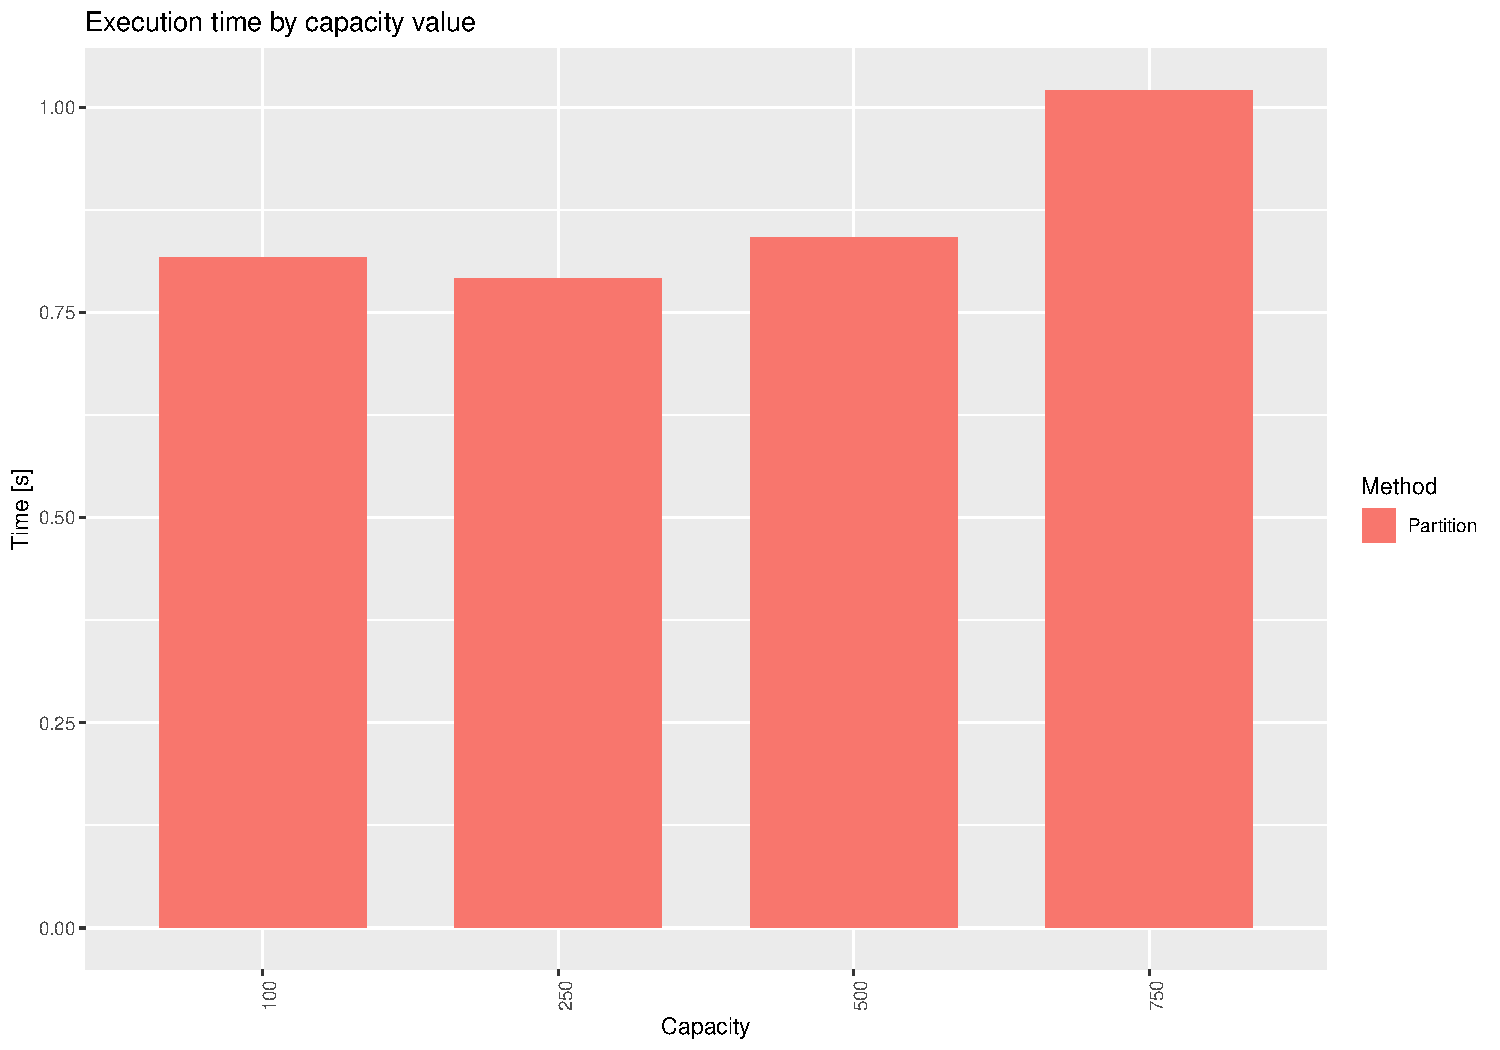
\includegraphics[width=0.8\textwidth]{figures/ByCapacity}
\end{frame}
\begin{frame}{Experiments}{Results}
    \centering
    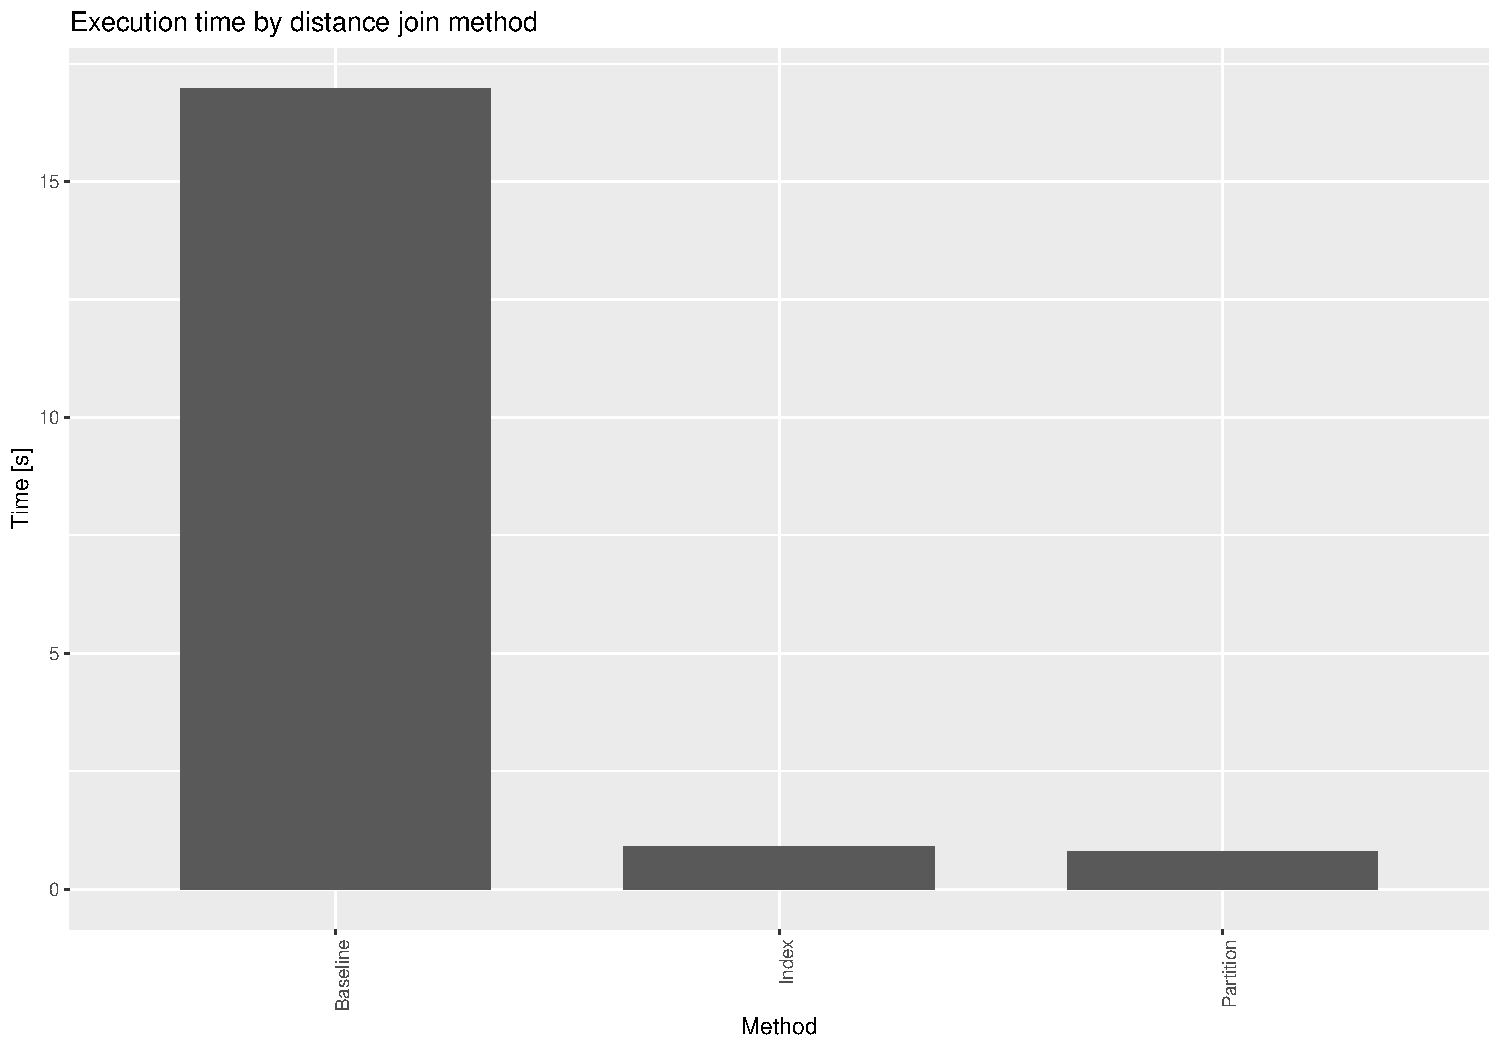
\includegraphics[width=0.8\textwidth]{figures/ByMethod1}
\end{frame}
\begin{frame}{Experiments}{Results}
    \centering
    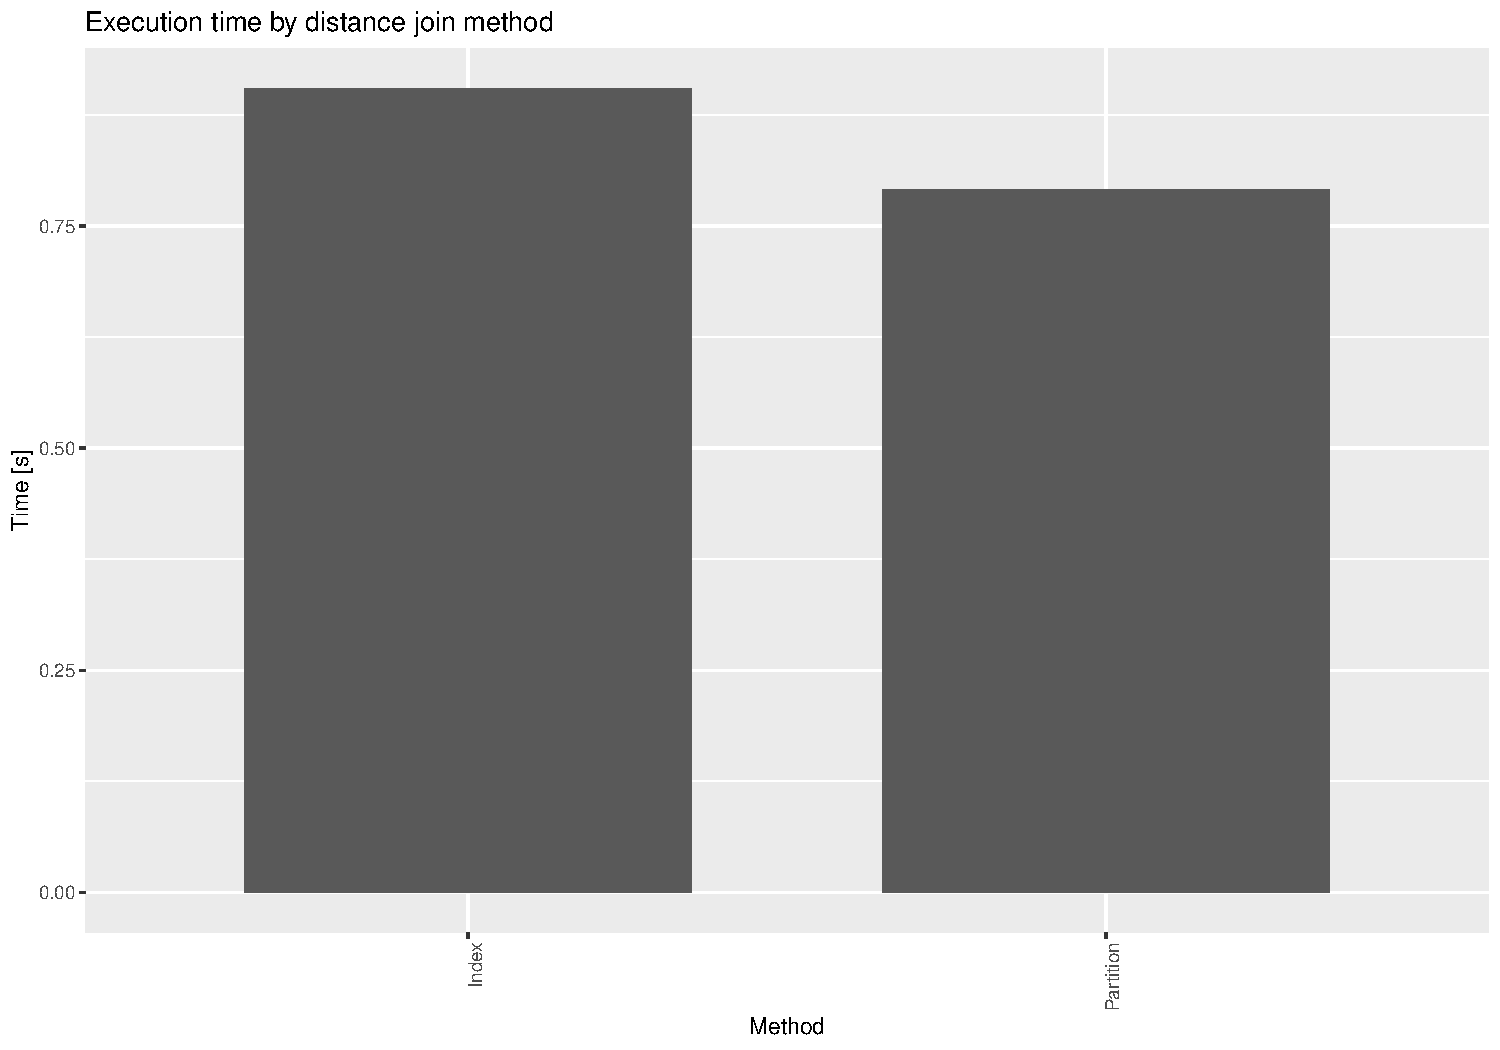
\includegraphics[width=0.8\textwidth]{figures/ByMethod2}
\end{frame}

\begin{frame}{What's next}
    \begin{itemize}
        \item Integrating the aproach to perform points vs centers join (taking advantage of the current local partitioning).
        \item Validate and test performance.
    \end{itemize}
\end{frame}

\end{document}

